\documentclass[a4paper,12pt]{report}            % [forma A4, taille police] {Type}
    \usepackage[utf8]{inputenc}                
    \usepackage[T1]{fontenc}                        % Codage des fontes TeX
    \usepackage[francais]{babel}
    \usepackage{graphicx}
    \usepackage{wrapfig}
    \usepackage{fancyhdr}
    \usepackage{xcolor}
    \usepackage{hyperref}
    \usepackage{listings}
    \usepackage{fullpage}
    \usepackage{eso-pic}
    \usepackage{titlesec}
    \titleformat{\chapter}[hang]{\bf\huge}{\thechapter}{2pc}{}
    \lstset {numbers=left ,stepnumber=1,firstnumber=0,numberfirstline=true}
    \hypersetup{
        bookmarks=true,         % show bookmarks bar?
        unicode=false,          % non-Latin characters in Acrobat’s bookmarks
        pdftoolbar=true,        % show Acrobat’s toolbar?
        pdfmenubar=true,        % show Acrobat’s menu?
        pdffitwindow=false,     % window fit to page when opened
        pdfstartview={FitH},    % fits the width of the page to the window
        pdftitle={My title},    % title
        pdfauthor={Author},     % author
        pdfsubject={Subject},   % subject of the document
        pdfcreator={Creator},   % creator of the document
        pdfproducer={Producer}, % producer of the document
        pdfkeywords={keyword1, key2, key3}, % list of keywords
        pdfnewwindow=true,      % links in new PDF window
        colorlinks=true,       % false: boxed links; true: colored links
        linkcolor=black,          % color of internal links (change box color with linkbordercolor)
        citecolor=green,        % color of links to bibliography
        filecolor=magenta,      % color of file links
        urlcolor=blue           % color of external links
    }
    
    \author{Samuel HUET \& Thomas COUTANT}
    \title{\huge{Les Antennes}}
    
    \begin{document}
\maketitle
\renewcommand{\contentsname}{SOMMAIRE} % Dans le corps du document,avant la commande \tableofcontents.
\tableofcontents

\chapter{Amplificateur}
\addcontentsline{toc}{chapter}{Amplificateur}

\section{Pertes}

Avant de pouvoir déterminer l'amplification de l'amplificateur, il est nécéssaire de déterminer la pertude dûs aux cables, 
Pour cela, nous utilisons le montage suivant :

\begin{center}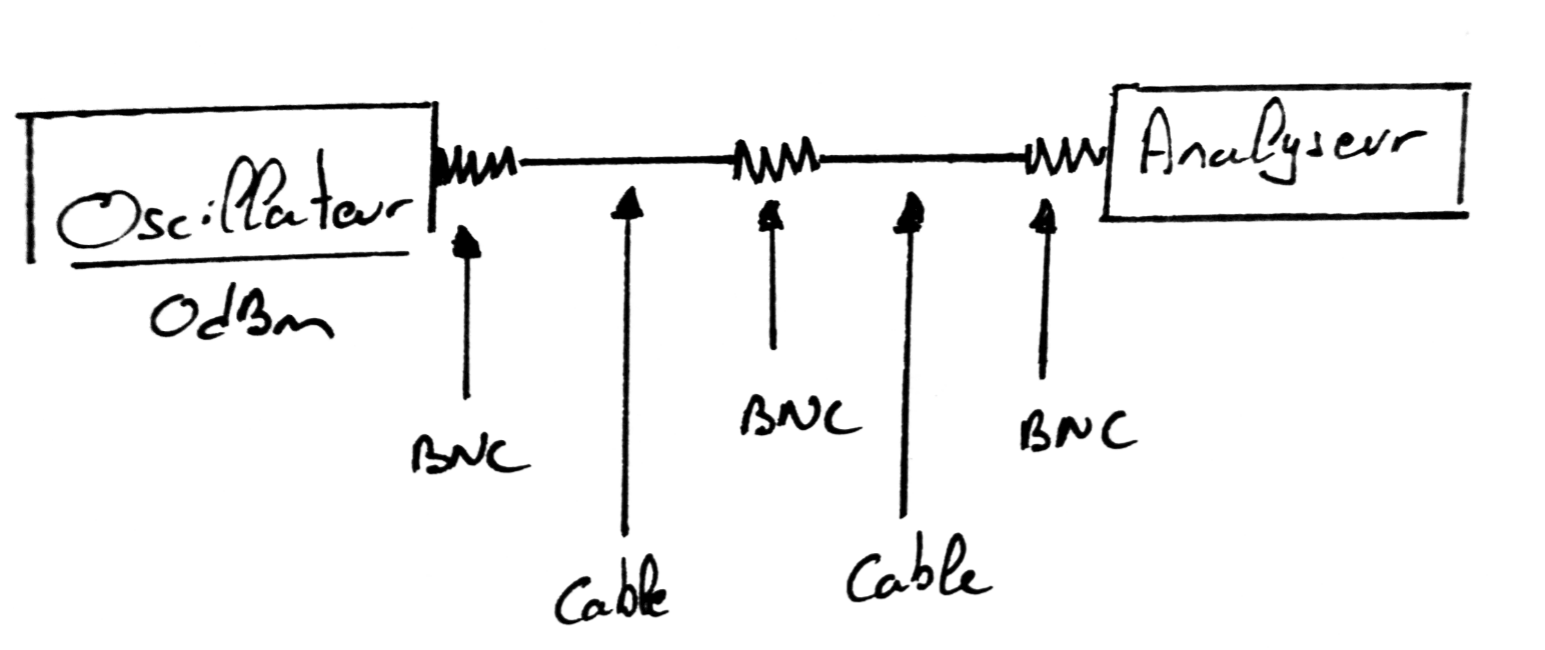
\includegraphics[scale = 0.2]{pic/mesure_perte.png}\\ \end{center}

Il est ainsi très facile, en visualisant l'analyseur de spectre de derterminer ces pertes.
Sur notre exemple, avec les cables coaxiaux utlisés, la perte de 4.2 dB, mais cela dépend évidemment du type de
materiel utilisé..

\chapter{WattMètre}
\addcontentsline{toc}{chapter}{WattMètre}

\chapter{Mesure d'antennes}
\addcontentsline{toc}{chapter}{Mesure d'antennes}

\chapter{Reception FM}
\addcontentsline{toc}{chapter}{Reception FM}

\chapter{Conclusion}
\addcontentsline{toc}{chapter}{Conclusion}
\end{document}